\subsection{Celdas de Combustible}

A pesar de que las celdas de combustible son una tecnología de hace más de un siglo y medio (desarrollada por primera vez por el físico galés Sir William Grove en 1842), hoy en día despiertan un particular interés en el campo de la generación renovable por su alta eficiencia, su dependencia en recursos obtenibles fácilmente de maneras ambientalmente amigables, y por la generación de agua como único deshecho.\\

Por estas razones se eligió trabajar con esta tecnología, particularmente con el tipo de celda más común hoy en día, las Celdas de Combustible de Membrana de Intercambio Protónico o PEMFC (del inglés \textit{Proton Exchange Membrane Fuel Cell}), cuyo funcionamiento se profundiza más adelante.\\

\subsubsection{Principio de Funcionamiento de las Celdas de Combustible}

Esencialmente, una celda de combustible es una celda galvánica o celda voltáica en la cual la energía libre de una reacción química redox (entre un combustible y un agente oxidante o \textit{comburente}) se convierte a energía eléctrica mediante una corriente y una diferencia de potencial$^{[FC-FundamentalsAndApplications]}$. En nuestro caso particular, el combustible es el hidrógeno molecular ($H_2$), el agente oxidante es el oxígeno ($O_2$) abundante en la atmósfera, y los productos son la energía eléctrica y el agua ($H_2O$) según indica la siguiente ecuación química balanceada.

\begin{equation}\label{redox_celda}
    2H_2\ +\ O_2\ \longrightarrow\ 2H_2O
\end{equation}

La estructura interna de una celda de combustible, visible en la figura \ref{fuel_cell}, consiste de un ánodo (electrodo negativo) al cual ingresan las moléculas de hidrógeno, un cátodo (electrodo positivo) en el que ingresa el oxígeno y se despide el agua, y un electrolito como como interfaz entre ánodo y cátodo. La carga es conectada entre el ánodo y el cátodo.

\begin{figure}[h]
    \centering
    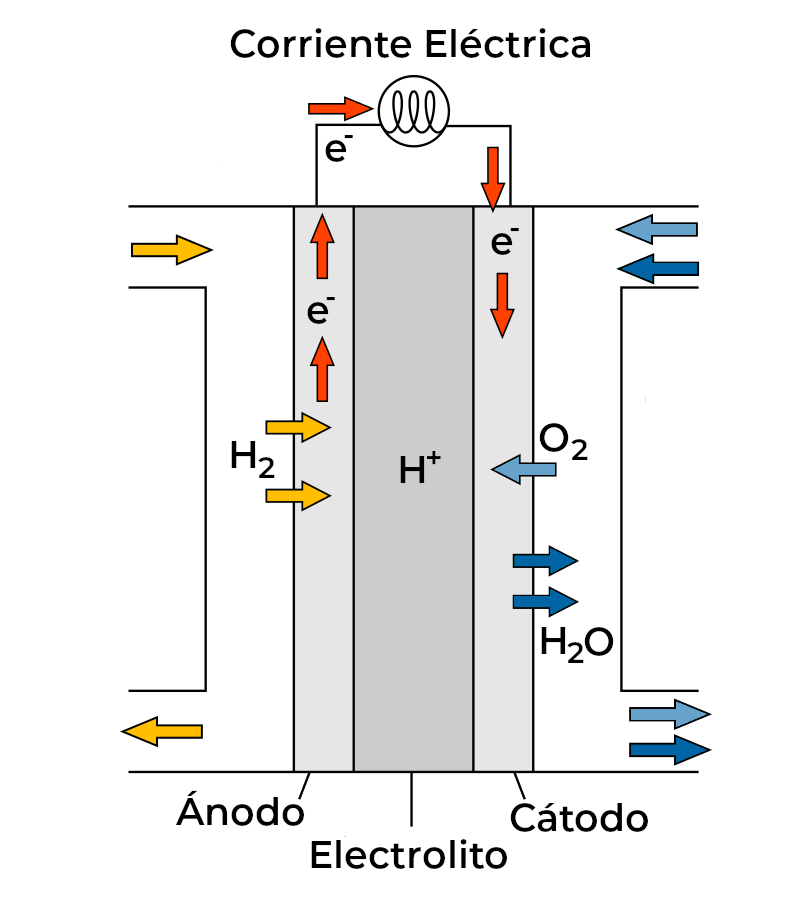
\includegraphics[scale=0.35]{Imagenes/Fuel Cell.png}
    \caption{Esquema de una celda de combustible, con todos sus componentes indicados (Placeholder).}
    \label{fuel_cell}
\end{figure}

La reacción redox de la ecuación \ref{redox_celda}, dentro de una celda de combustible como la del esquema, en realidad se separa en dos reacciones parciales distintas:

\begin{equation}\label{redox_anodo}
    2H_2\ \longrightarrow\ 4H^{+}\ +\ 4e^-
\end{equation}

\begin{equation}\label{redox_catodo}
    4H^{+}\ +\ 4e^-\ +\ O_2\longrightarrow\ 2H_2O
\end{equation}

De esta manera, alimentado simultáneamente el terminal negativo con combustible (hidrógeno) y el terminal positivo con oxidante (oxígeno) se producen las dos reacciones en las superficies de contacto del electrolito:

\begin{itemize}
    \item \textbf{En el ánodo} las moléculas de $H_2$ pierden sus electrones, bifurcándose los iones positivos de hidrógeno ($H^{+}$) por el electrolito y los electrones libres a través de la carga (ecuación \ref{redox_anodo}). Es una reacción exotérmica (libera calor) que resulta en el calentamiento de la celda.
    \item \textbf{En el cátodo} los iones $H^{+}$ del electrolito, los electrones libres, y las moléculas de oxígeno reaccionan para formar como producto el agua (ecuación \ref{redox_catodo}).
\end{itemize}

Mediante este proceso electroquímico se generan dos corrientes distintas: una corriente interna de iones $H^{+}$ (cargas positivas) en el electrolito, desde el ánodo hacia el cátodo; y una corriente externa de electrones $e^-$ (cargas negativas) circulando por la carga, en el mismo sentido que la corriente de iones. Esta última corriente de electrones es la que nos resulta útil para poder alimentar algún tipo de carga.\\

\subsubsection{De Celda a Pila de Combustible}

Sin embargo, una celda de combustible individual como en la figura \ref{fuel_cell} no es capaz de entregar una diferencia de potencial lo suficientemente alta para la gran mayoría de las aplicaciones, con una tensión de celda común situada entre 0.7 V y 1.3 V, dependiendo de varios aspectos constructivos específicos de la celda.\\

Entonces, para obtener un dispositivo con una tensión de salida de niveles utilizables, esta tecnología generalmente se comercializa en forma de pilas o \textit{stacks} de celdas individuales conectadas en serie como se ve en la figura \ref{fuel_cell_stack}, generalmente de entre diez y cien celdas, cuya tensión es la suma de la tensión de cada celda que la compone.\\

Esto se logra, como dice su nombre, apilando todas las celdas de combustible para formar el \textit{stack}, utilizando placas de interconexión para conectar electrodos de polaridad opuesta de dos celdas aledañas (es decir, se conecta el ánodo de una celda con el cátodo de la siguiente); además de cumplir la función de aislar el combustible de una celda del agente oxidante de la celda contigua. Este es el tipo de conexionado de celdas más común, llamado \textit{Planar-Bipolar Stacking} o Apilado Planar-Bipolar$^{[FCHandbook]}$.

\begin{figure}[H]
    \centering
    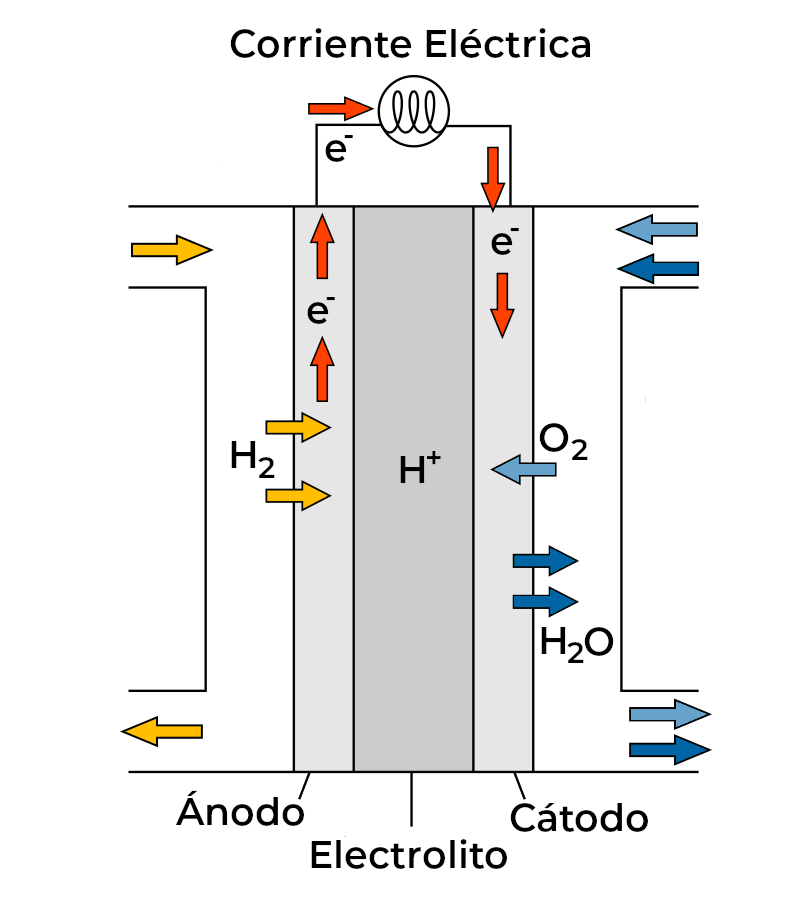
\includegraphics[scale=0.2]{Imagenes/Fuel Cell.png}
    \caption{Figura de un stack de celdas.}
    \label{fuel_cell_stack}
\end{figure}

\subsubsection{Aspectos Constructivos de Celdas}

Habiendo repasado el principio básico de funcionamiento de las celdas de combustible, ahora se realizará una breve descripción de los aspectos constructivos de las mismas. La utilización de distintos materiales y composiciones de las partes que las componen derivan en distintos tipos de celdas, que, a pesar de funcionar bajo el mismo principio básico, poseen cada una sus ventajas y desventajas que las hacen más o menos apropiadas para distintas aplicaciones.\\

Como las reacciones químicas ocurren en superficies microscópicas dónde alguno de los electrodos está en contacto con el electrolito, generalmente los electrodos se fabrican de materiales porosos que aumentan la posible superficie de contacto entre ambas fases, acelerando las reacciones necesarias para producir energía. Sin embargo, en muchos casos, a temperaturas bajas los materiales de los electrodos no son capaces de producir la suficiente actividad electroquímica, por lo que suelen agregarse pequeñas cantidades de catalizador en las zonas de contacto para acelerar la reacción.\\

En tanto al electrolito, estos suelen estar hechos de materiales en estado líquido o sólido, dependiendo del tipo de celda, pero siempre deben tener una alta conductividad de iones positivos, de manera que los iones $H^{+}$ circulen solo por el elctrolito y no por el circuito externo. Adicionalmente, este material debe actuar de barrera física para evitar que se mezclen los flujos de combustible y comburente.\\

En tanto a la geometría de las celdas, se ha expermientado con una gran variedad de formas para los electrodos y electrolitos pero, hoy en día las pilas que se producen son mayormente planas, y en algunos casos tubulares.\\

\subsubsection{Tipos de Celdas}

Hay muchas formas de clasificar las distintas tecnologías de celdas, pero en nuestro caso nos vamos a enfocar en la distinción más común, que es la clasificación según el material usado como electrolito. Hoy en día, hay seis tipos distintos de celdas segun electrolito, descritas a continuación, con una mayor profundización mayor en las del tipo PEMFC que se mencionaron anteriormente, ya que son este tipo de pilas las que nos interesa en nuestra aplicación particular.

\begin{itemize}
    \item \textbf{Celda de Combustible Alcalina (AFC)}\\
    Hola
    \item \textbf{Celda de Combustible de Metanol Directo (DMFC)}\\
    Hola
    \item \textbf{Celda de Combustible de Ácido Fosfórico (PAFC)}\\
    Hola
    \item \textbf{Celda de Combustible de Carbonato Fundido (MCFC)}\\
    Hola
    \item \textbf{Celda de Combustible de Óxido Sólido (SOFC)}\\
    Hola
    \item \textbf{Celda de Combustible de Membrana de Intercambio Protónico (PEMFC)}\\
    Hola
\end{itemize}